% Chapter 1

\chapter{Introduction} % Main chapter title

\label{Chapter1} % For referencing the chapter elsewhere, use \ref{Chapter1} 

\lhead{Chapter 1. \emph{Introduction}} % This is for the header on each page - perhaps a shortened title

%----------------------------------------------------------------------------------------

%----------------------------------------------------------------------------------------
\section{About the report}
\label{sec:about}
The aim of this report is to introduce the topic of Imaging in Radio Astronomy to students with a background in signal \& image processing and having a general knowledge of physics. This was done so that the reader would acquire the basic knowledge about what is done actually, the practical issues, and thus those interested to learn or try out things on their own on the topic would be encouraged to read the literature referred to.\\

The report is composed of 4 main chapters,
\textit{chapter 1} is an introduction to the field, the main goals people aim for in the area and it also stands as a basis for the other chapters. Then \textit{Chapter 2} continues more thoroughly on the topic of cross-correlation, and we pass on to \textit{chapter 3} which deals more with theorems, sampling considerations, data calibration, and image reconstruction/retrieval, generally things related to linear processes. Then finally \textit{chapter 4} expounds about the actual processing of the raw image with enhancing techniques which usually deal with non-linear processes. So we hope that the reader will find this small piece of work that we put together very fluent and comprehensive on the topic.

\section{The pioneers}
\label{sec:pioneers}
\begin{wrapfigure}[10]{r}{0.3\textwidth}

  \begin{center}
    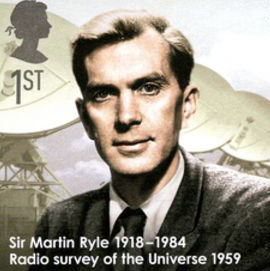
\includegraphics[scale= 0.45]{Figures/Sir-Martin-Ryle-C}
  \end{center}
  
 	\caption[Sir Martin Ryle]{\\Sir Martin Ryle}
	\label{fig:Martin}
	
\end{wrapfigure}

As Assoc. Prof. R. Somanah usually says, one cannot talk about Radio Imaging without mentioning a main pioneer in the field, Sir Martin Ryle. He was a British radio astronomer who did develop revolutionary radio telescopes systems and used them for the accurate location and imaging of weak radio sources. Earlier he worked on the study of radio waves from the Sun and sunspots, and later discovered the first quasi-stellar object known as the Quasar \textbf{\textit {Explanation Ruben}}. Martin Ryle and his colleague Anthony Hewish were the first \textbf{astronomers} to ever receive the Nobel prize in Physics in 1974 for their overall contribution to \textbf{radio astronomy}. 
%Make a foot note and improve this section about Quasars
%http://colnect.com/en/stamps/stamp/184650-Sir_Martin_Ryle_-_Radio_Surveyor_of_the_Universe-Eminent_Britons-United_Kingdom_of_Great_Britain_Northern_Ireland

\section{Introductory basic concepts}
\subsection{Imaging by Interferometry in R.A.}
\label{sec:intIntro}
\begin{figure}[htbp]

  \begin{center}
    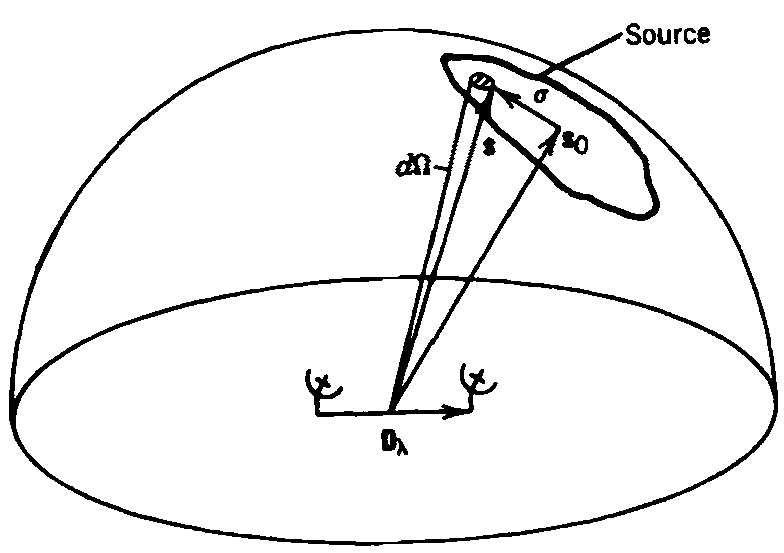
\includegraphics[scale= 1.3]{Figures/sSource}
  \end{center}
  
 	\caption[Diagrammatic representation of an elementary radio interferometer setup]{\\ A Radio interferometer setup diagrammatic representation}
	\label{fig:RadioIntSphere}
	
\end{figure}
Interferometry is a technique where electromagnetic waves are superimposed in order to extract information about the waves. As concern Radio Astronomy when at least 2 radio telescopes are working in tandem, the setup is given the name of radio interferometer. Radio Telescopes are actually antennas which basically are devices that respond to incoming electromagnetic radiation and output electrical currents related to this reponse.
For application in Radio Astronomy passive radio telescopes i.e. receiving antennas are used.
\begin{figure}[htbp]

  \begin{center}
    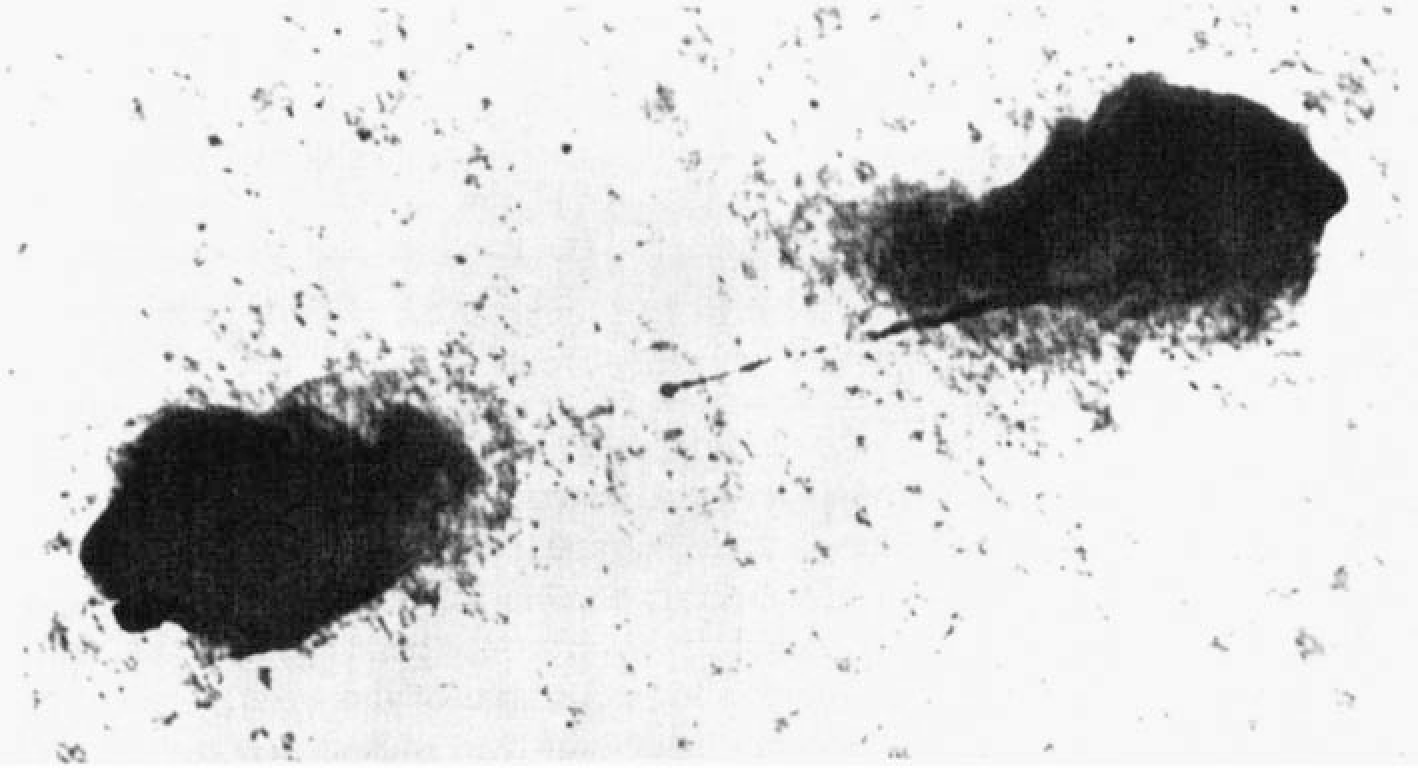
\includegraphics[scale= 0.75]{Figures/cynus_A}
  \end{center}
  
 	\caption[Cygnus A]{\\Cynus A}
	\label{fig:CygnusA}
	
\end{figure}
\subsection{Why are radio interferometers used?}
\label{sec:intReason}
\begin{figure}[hbp]

  \begin{center}
    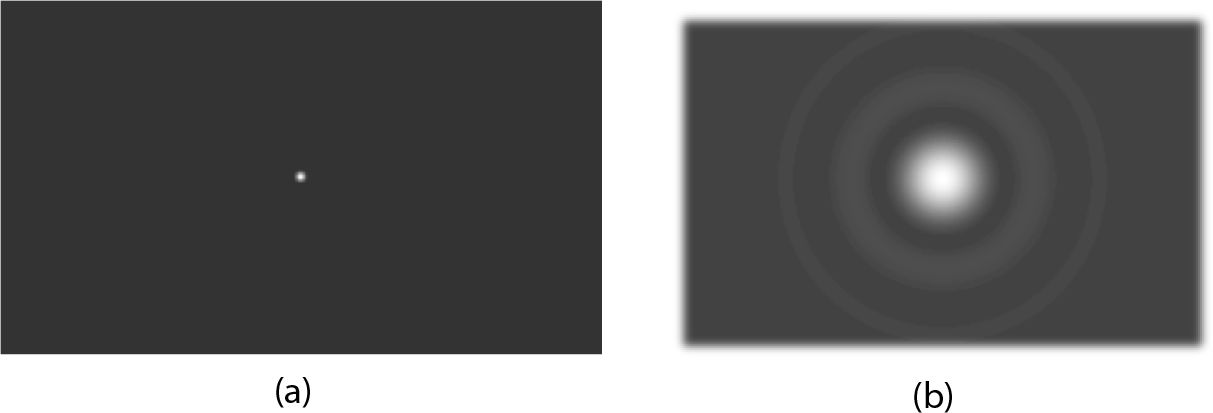
\includegraphics[scale= 1]{Figures/AntennaDif}
  \end{center}
  
 	\caption[Diffraction Effect]{\\Diffraction Effect}
	\label{fig:DifPat}
\end{figure}

To answer this question one must introduce the concept of angular resolution, the latter describes the angular distance between two point sources that can be differentiated by an aperture. Because of the diffraction effect, an antenna pattern has side lobes,
which are sensitive to sources outside the main antenna beam, limiting resolution. 
\begin{figure}[htbp]

  \begin{center}
    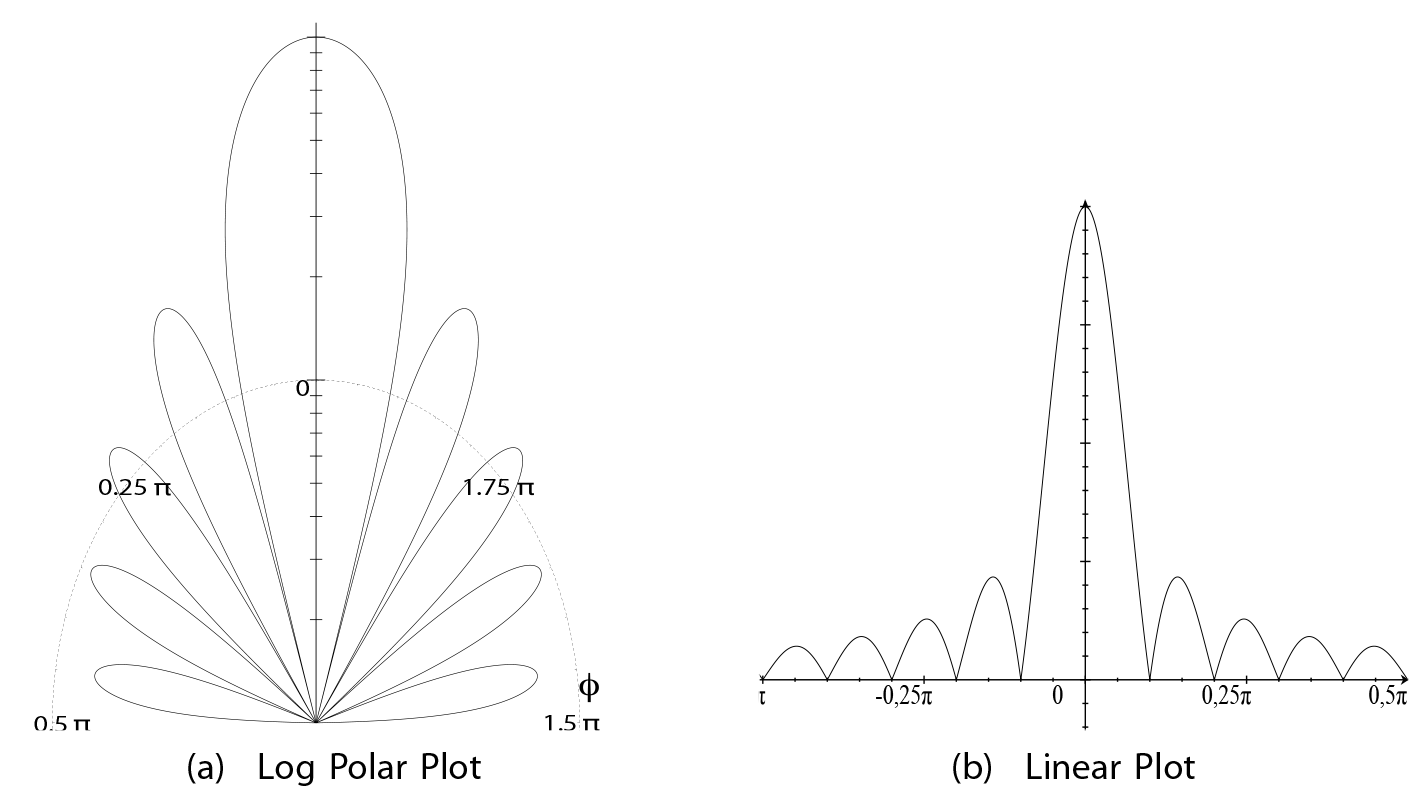
\includegraphics[scale= 1]{Figures/AntennaPattern}
  \end{center}
  
 	\caption[Antenna Pattern]{\\Antenna Pattern}
	\label{fig:AntPat}
\end{figure}
When a planar electromagnetic wave enters an aperture, the electromagnetic wave is distorted in what is called a diffraction pattern. Therefore a finite sized aperture cannot correctly record the radio brightness without some distortion of the original signal. The diffraction distortion is due to the interaction of the original EM wave with the edges of a finite sized aperture, which creates the fringe pattern of destructive and constructive interference. Diffraction effects all types of EM waves when entering an aperture, but is more severe for longer wavelengths. The distance to the first zero of the diffraction pattern of a circular aperture is given by
\begin{equation}
R \simeq 1.22\frac{\lambda}{D} 
\end{equation}
\begin{figure}[htbp]

  \begin{center}
    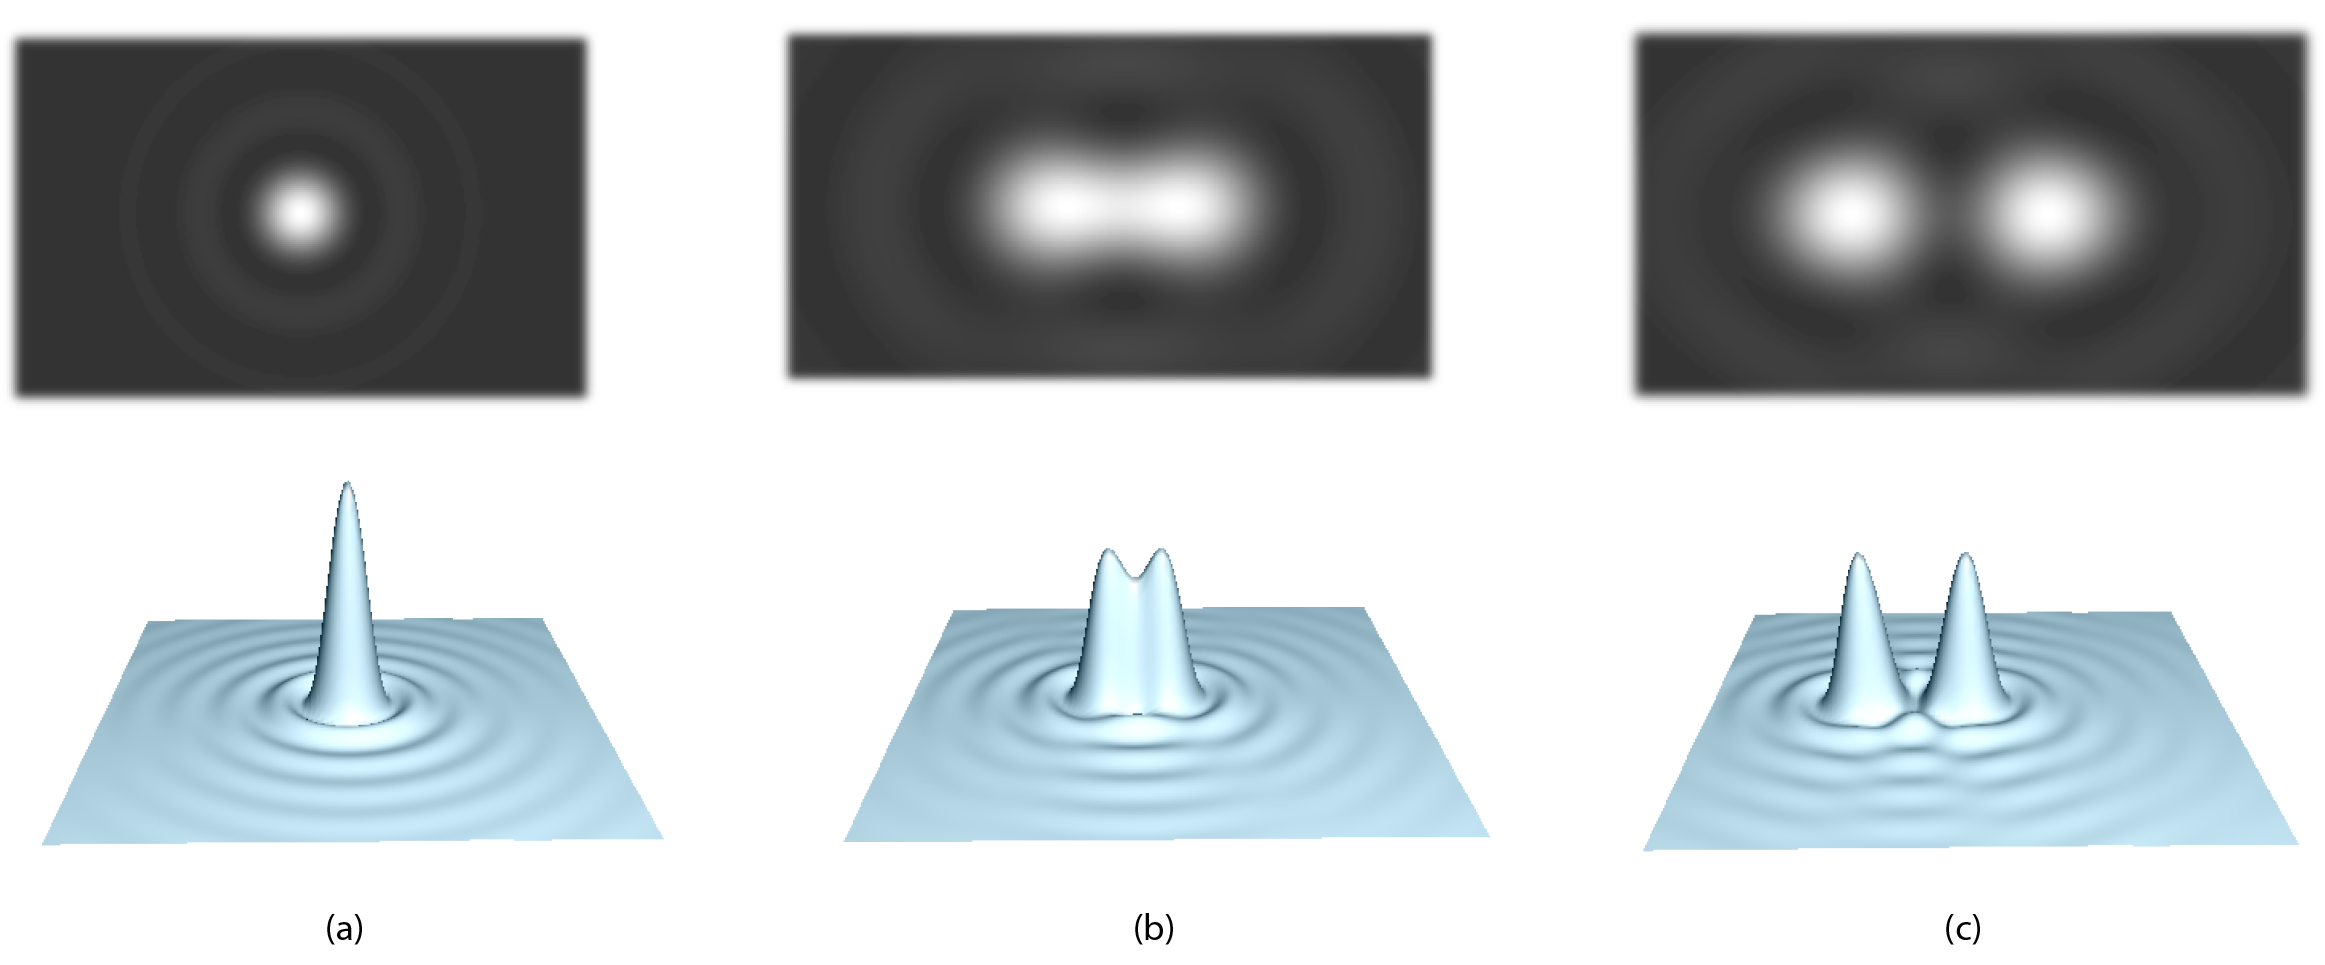
\includegraphics[scale= 0.75]{Figures/angres}
  \end{center}
  
 	\caption[Angular Resolution]{\\Angular Resolution}
	\label{fig:Ang}
\end{figure}
If two objects are closer than the first minima, for a particular
aperture, they cannot be distinguished. Therefore the first minima, determines the resolving
capabilities of an aperture and is called the angular resolution $R$. The angular
resolution, represented in the right-hand side of the equation, depends on both the wavelength
and the aperture diameter. As a consequence of dealing with radio waves, which have a long
wavelength, radio astronomy requires large telescopes in order to improve the resolution and
produce detailed images (radio brightness readings). The dimensions of a single radio aperture needed to meet the angular resolution requirements are extremely impractical in terms of strict design requirements and physical constraints. For example, to achieve the same angular resolution as the naked human eye, a radio antenna’s aperture observing a source at 4GHz must be 750m in diameter. Therefore the way this issue is coped for is by using a radio interferometer setup, in the latter case its effective aperture diameter now corresponds to the largest separation of the 2 telescopes and actually a much better resolution can be obtained more easily, as one can have telescopes with a desired distance between them (in that small calculation $\sim$ 750m) which is more practical than having to build a single radio telescope with a large aperture diameter. This is from that fact that the technique is coined \textit{Aperture Synthesis} as with that setup the aperture diameter and in consequence the resolution of a much larger telescope can be emulated by the aforementioned mean.  Knowing the impulse response of an aperture, a closer reconstruction of the original source can be made by performing a deconvolution, this will be discussed in \textit{chapter 4}
%Reference Andrew Woods' MSc Thesis
\newpage
\subsection{The principle of a radio Interferometer}
\label{sec:intPrincipia}
Consider the figure~\ref{fig:RadioSet} below which shows the direction of incoming electromagnetic planar wavefronts received at the antenna from the sky.
\begin{figure}[htbp]
\center
    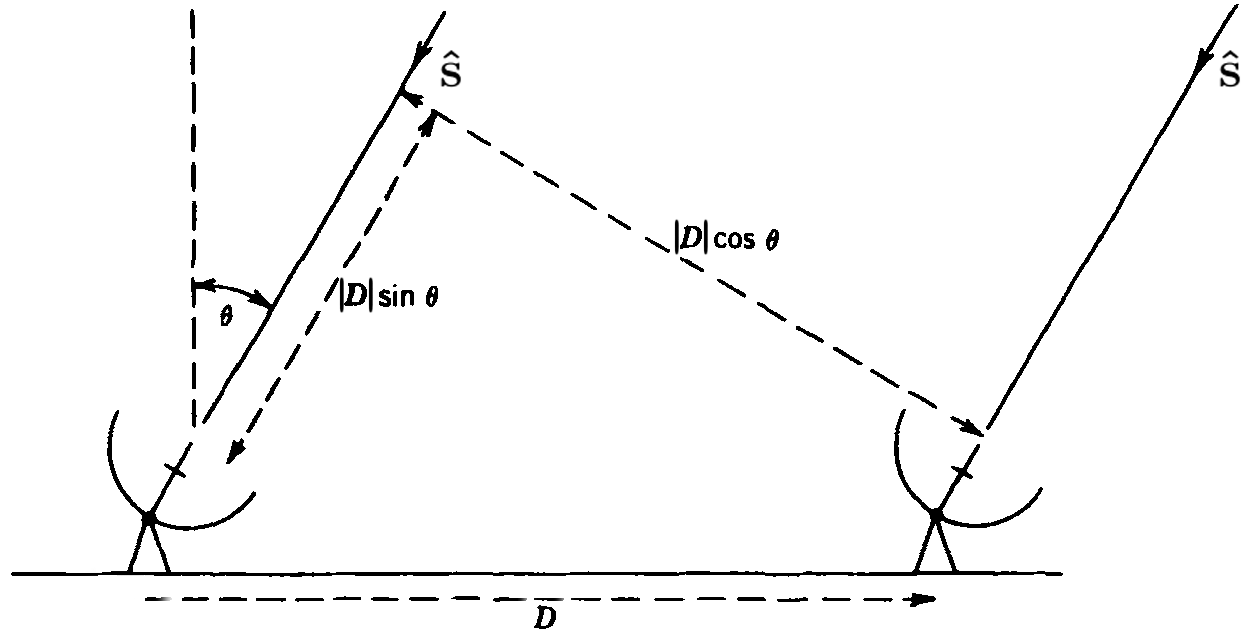
\includegraphics[scale= 0.9]{Figures/RadioSet}
 	\caption[An elementary interferometer]{\\Geometry of an elementary interferometer}
	\label{fig:RadioSet}
\end{figure}
Depending on the direction of the wavefront relative to the direction the antennas point to, here characterised by the angle $\theta$, the same wavefront from the sky will reach a particular antenna first, here the right one, or both would get the same wavefront at the same time, in the first case it is only after a certain lapse of time that the wavefront reaches the other antenna, the left one. The extra distance the wavefront has to travel to reach the left antenna is the projection of the baseline direction on the unit vector in the source direction which is equal to ${\bf D}\cdot \hat{\bf s}$.

\begin{equation}
{\bf D}\cdot\hat{\bf s} = |{\bf D}|\cdot\cos(90^{\circ} - \theta)= |{\bf D}|\sin(\theta)
\end{equation}
This is also the extra time that the wavefront takes at speed of light to reach the left antenna known as the geometric delay or time delay. The geometric delay, $\tau_{g}$ is thus the following,
\begin{equation}
\tau_{g}=  \frac{{\bf D}\cdot {\bf \hat{s}}}{\textrm{c}}     
\end{equation}
where, c, is the speed of light in vacuum.

As mentioned in section~\ref{sec:intIntro} antennas output electrical signals in response to the incoming wavefront, thus it is quite obvious that the signal output at the left antenna would be similar to that from the the right antenna but delayed by the geometric delay. Therefore, what we do in radio interferometry is that we have a measure to characterise this antenna pair - signal relationship in response to the EM radiation from a direction in the sky and it is called the \textbf{visibility}.
The relationship between the visibility and what is observed is direct. So one can make a map of the visibility and be able to have information about the sky observed and this is discussed further in the section  section~\ref{sec:intVisInt}
\subsection{A free coordinate system}
\label{sec:intFreeCoor}
Before we continue further let us first use an adequate coordinate system that will be the basis of our subsequent discussion.
\begin{figure}[htbp]
\center
    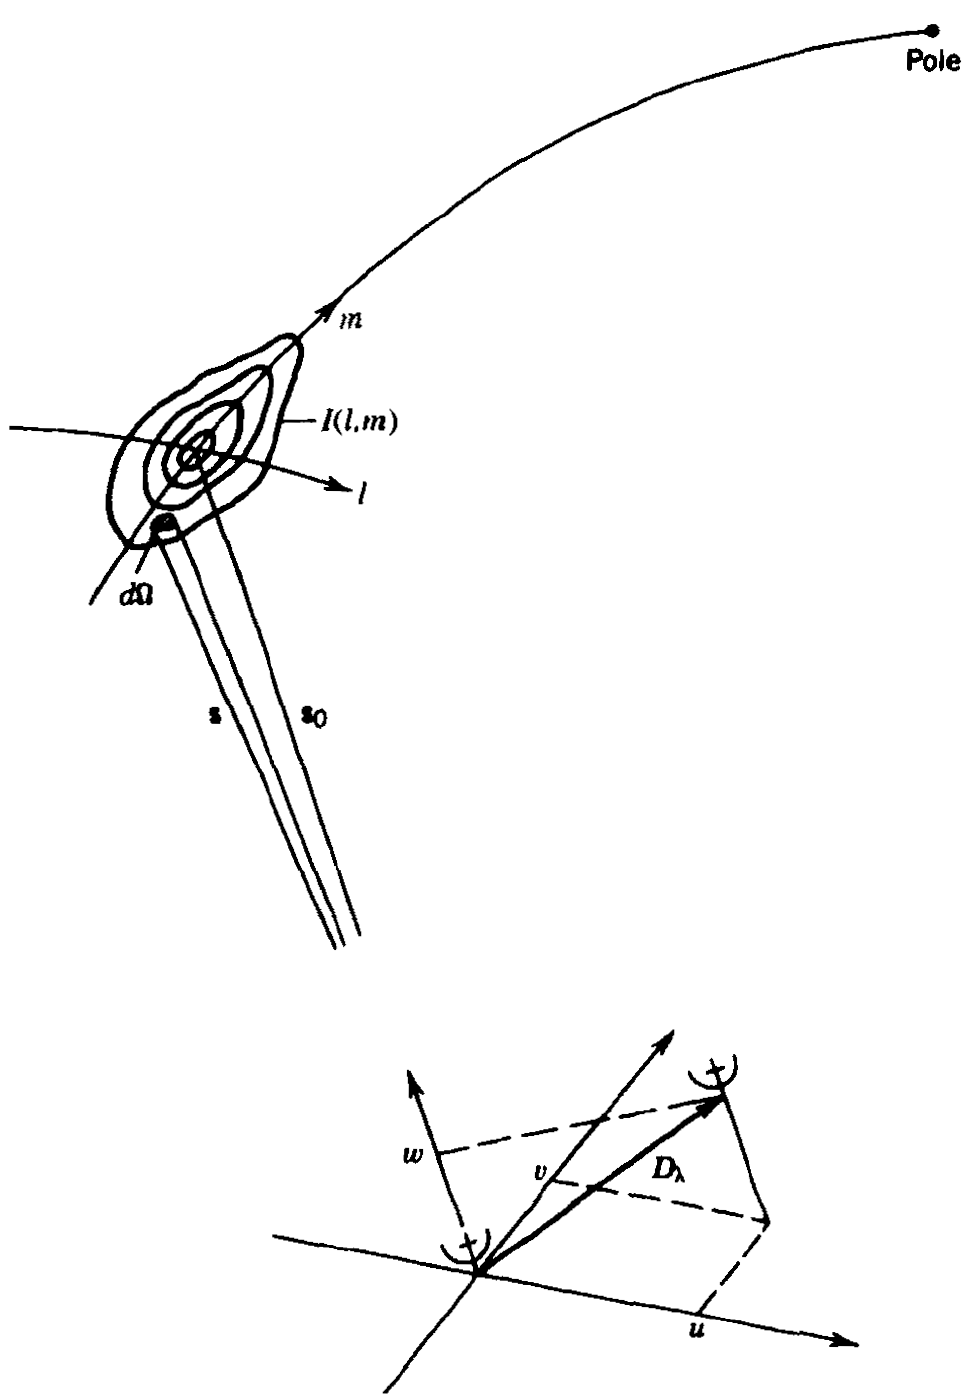
\includegraphics[scale= 0.9]{Figures/freeCoor}
 	\caption[Free coordinate system]{\\Free coordinate system}
	\label{fig:freeCoor}
\end{figure}
Consider the figure~\ref{fig:freeCoor}.
Suppose that the antennas track the source under observation, which is the most common situation, and let the unit vector $\bf{s_0}$ indicate the phase reference position. This position, known as the phase-tracking center, becomes the center of the field to be mapped. The magnitude of the baseline vector is
measured in wavelengths at the center frequency of the observing band, and the baseline direction has components $(u, v , w)$ in a right-handed coordinate system, where $u$ and $v$ are measured in a plane normal to the direction of the phase reference position. The spacing component $u$ is measured toward the north as defined by
the plane through the origin, the source, and the pole, and $v$ toward the east. The component $w$ is measured in the direction ${\bf\hat{s}_0}$. Source direction or position on the celestial sphere have the components $(l,m,n)$ which are simply the respectively the direction cosines of the particular direction/position ${\bf \hat{s}}$ in terms of the $(u,v,w)$ components i.e. 
\begin{equation}
{\bf \hat{s}} = (l,m,n) = (\hat{\bf s}\cdot\hat{\bf u},\hat{\bf s}\cdot\hat{\bf v},\hat{\bf s}\cdot\hat{\bf w})
\end{equation}
Then since $l^2 + m^2 + n^2 = 1$ we can re-express $n$ in terms of $l$ and $m$ as folllows, 
\begin{equation}
n = \sqrt{1 - l^2 - m^2}
\end{equation}
leading us to re-express source directions with the following components i.e.
\begin{equation}
{\bf \hat{s}} = (l,m, \sqrt{1 - l^2 - m^2})
\end{equation}
\begin{figure}[htbp]
\center
    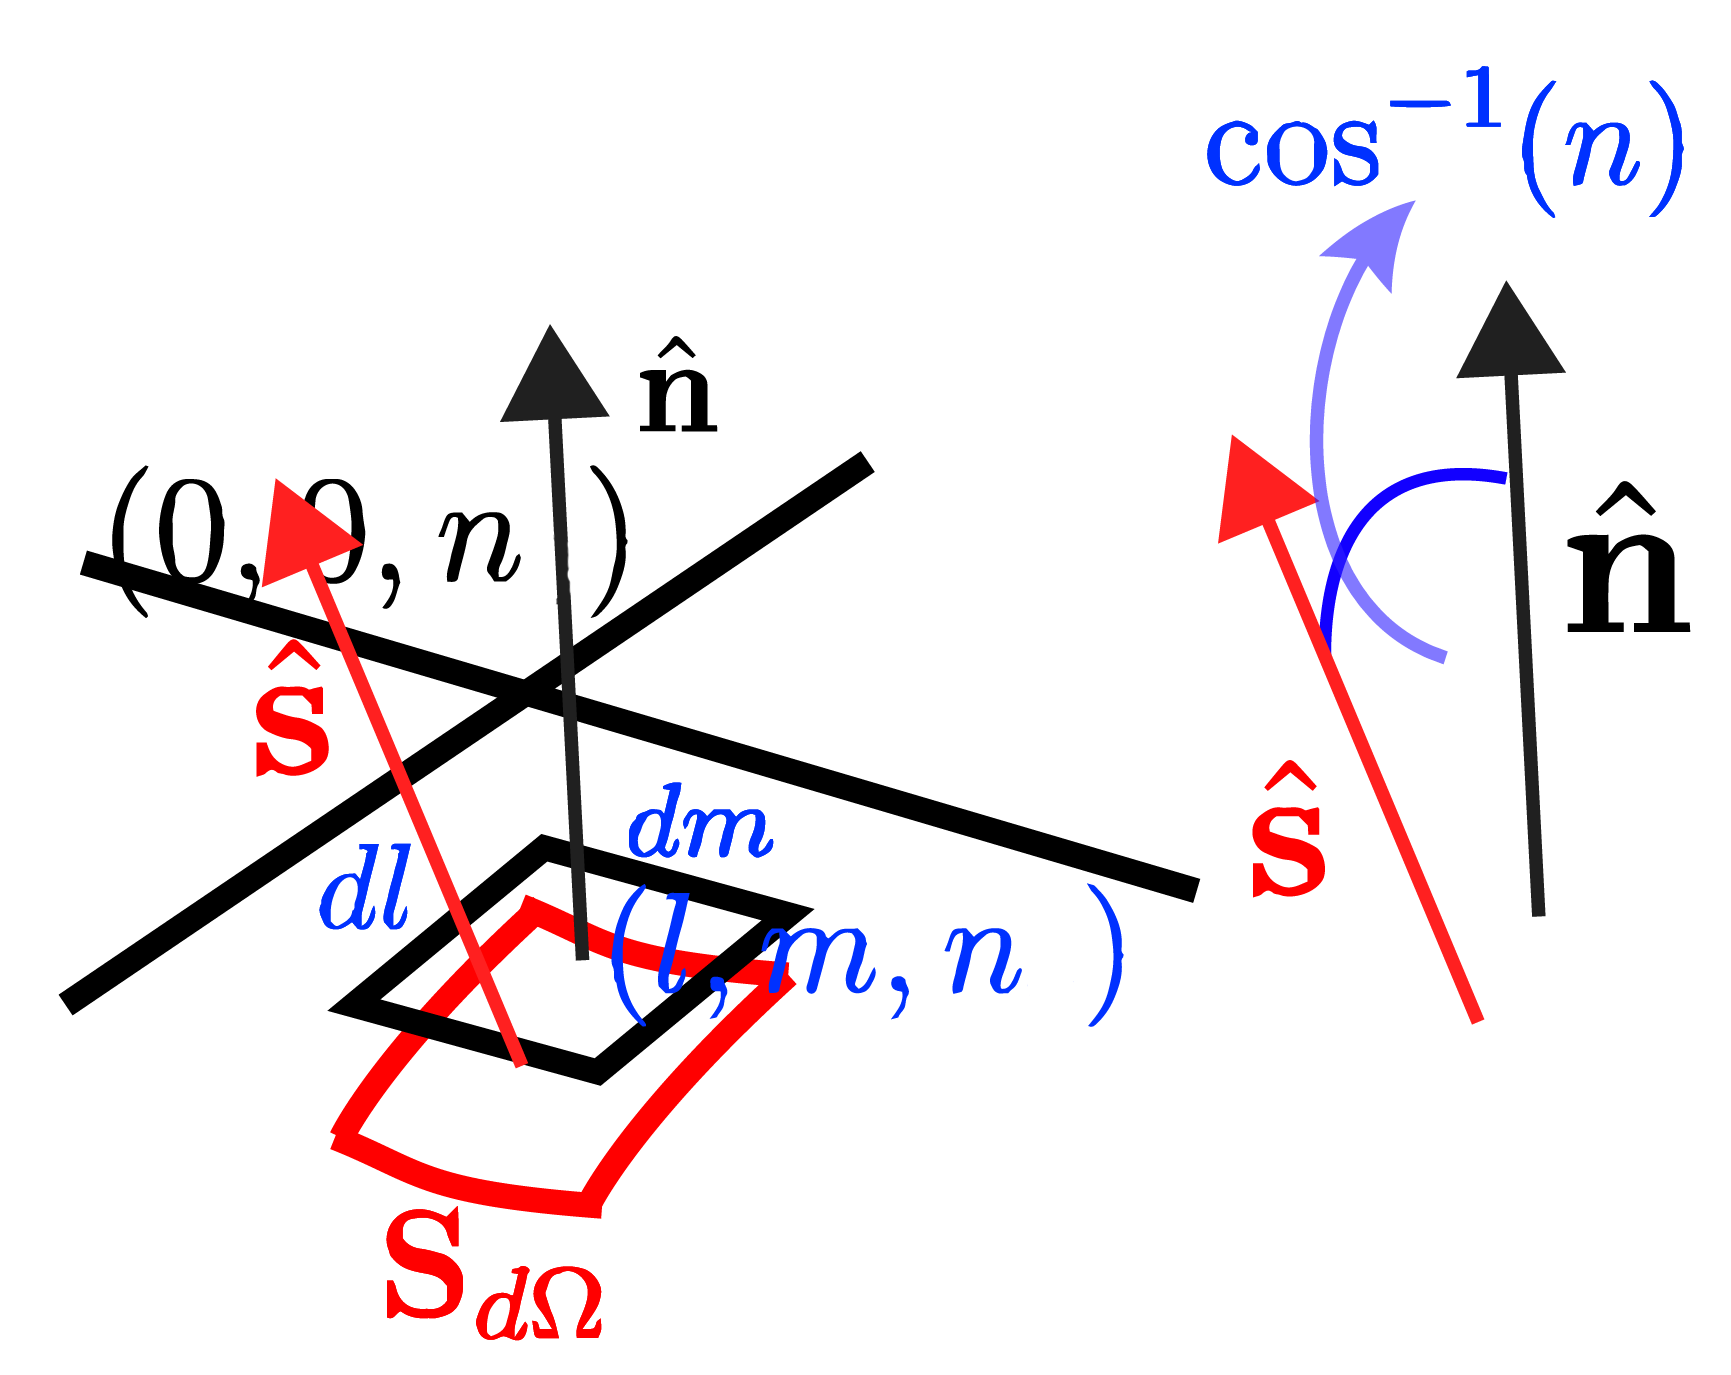
\includegraphics[scale= 0.5]{Figures/sAngle}
 	\caption[Element of Solid Angle]{\\Element of Solid Angle}
	\label{fig:sAngle}
\end{figure}
\begin{equation}
dl \quad dm \quad \hat{\bf s} \quad \hat{\bf n} \quad \cos^{-1}(n)
\end{equation}

\begin{equation}
{\bf S}_{dldm} = S_{dldm}\cdot\hat{\bf n} \quad {\bf S}_{d\Omega} = 
\end{equation}
\begin{equation}
(0,0,n_{0}) \quad (l,m,n_{0})
\end{equation}

\subsection{Visibility -- Sky intensity distribution relationship}
\label{sec:intVisInt}